\subsection{RTC}
\label{subsec:RTC}
Im vergangenen Kapitel (MCU) wurden bereits RC-Oszillatoren und Quarze erwähnt. Die RTC (Real Time Clock) beinhaltet ebenfalls einen Quarz, weshalb die RTC in diesem Kapitel näher erläutert wird.
Die RTC wurde bereits während des Projekt 5 integriert und in dessen Fachbericht dokumentiert. Nachfolgender Text wurde übernommen, damit die Vollständigkeit gewahrt wird.

\subsubsection{RTC - Projekt 5}
Um die gewonnenen Messdaten mit einem Zeitstempel zu versehen, wird eine \textbf{RTC} (\textit{real time clock}) benötigt. Um eine möglichst kleine Abweichung zu haben, wird eine hohe Präzision vorausgesetzt. Ausserdem soll die \textbf{RTC} über das in Kapitel \ref{chap:Interfaces} erwähnte \textbf{I$^2$C}-Bus angesteuert werden. Aus diesen Gründen wurde der \textbf{DS3231} implementiert, da dieser als Präzisions-\textbf{I$^2$C}-\textbf{RTC} die Anforderungen erfüllt. Die hohe Präzision des \textbf{DS3231} wird mit einem internen Temperatursensor erreicht, welcher Temperaturbedingte Abweichungen des Oszillators kompensiert. Zu sehen ist der \textbf{DS3231} mit seinen Anschlüssen in Abbildung \ref{fig:DS3231}.

\begin{figure}[h]
\centering
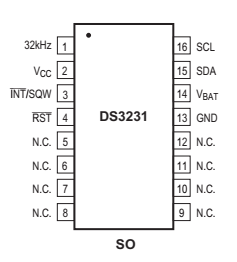
\includegraphics[width=0.4\linewidth]{graphics/DS3231.png}
\caption{\textbf{DS3231} mit seinen Anschlüssen \cite{DS3231DS}.}
\label{fig:DS3231}
\end{figure}

Die Anschlüsse des \textbf{DS3231} sind \textbf{VCC}, \textbf{GND}, \textbf{SCL}, \textbf{SDA}, \textbf{BAT}, \textbf{32K}, \textbf{SQW} und \textbf{RST}. \textbf{VCC} und \textbf{GND} werden für die Speisung benötigt. \textbf{SCL} und \textbf{SDA} sind Anschlüsse für den \textbf{I$^2$C}-Bus. \textbf{BAT} ist der positive Anschluss der Knopfbatterie, worüber deren Zustand kontrolliert werden, etwas anderes gespiesen oder eine andere Battery als Backup angeschlossen werden kann. \textbf{32K} ist ein Anschlusspin um den Output des 32kHz-Oszillators des \textbf{RTC} abzugreifen, was jedoch nicht verwendet wird. \textbf{SQW} ist ein zusätzlicher Output- oder Interrupt-Pin, welcher jedoch auch nicht verwendet wird. \textbf{RST} wird verwendet, um ein externes Element zu reseten oder als Indikator wenn die Hauptspeisung unterbrochen wird. \cite{DS3231DS}\\

\newpage
Die relevanten Spezifikationen des Chips sind in Tabelle \ref{tab:DS3231} aufgelistet.\\

\begin{table}[h]
\begin{tabular}{llllll}
\hline 
\textbf{Parameter} & \textbf{Min.} & \textbf{Typ.} & \textbf{Max.} & \textbf{Einheit} & \textbf{Condition} \\ 
\hline 
VCC & 2.3 & 3.3 & 5.5 & V &  \\ 
VBAT & 2.3 & 3 & 5.5 & V &  \\ 
Active Supply Current &  &  & 200 & $\mu$A & 3.63 V \\ 
 &  &  & 300 & $\mu$A & 5.5 V \\ 
Standby Supply Current &  & & 110 & $\mu$A & 3.63 V \\ 
 &  &  & 170 & $\mu$A & 5.5 V \\ 
Crystal Aging &  & $\pm$ 1 &  & ppm & First Year \\ 
 &  & $\pm$ 5 &  & ppm & 0-10 Years \\ 
Active Battery Current &  &  & 70 & $\mu$A & 3.63 V \\ 
 &  &  & 150 & $\mu$A & 5.5 V \\ 
Timekeeping Battery Current &  & 0.84 & 3 & $\mu$A & 3.63 V \\ 
 &  & 1 & 3.5 & $\mu$A & 5.5 V \\ 
\hline 
\end{tabular} 
\caption{Spezifikationen des \textbf{DS3231} \cite{DS3231DS}.}
\label{tab:DS3231}
\end{table}

Tabelle \ref{tab:DS3231} zeigt die für das Projekt relevanten Spezifikationen des \textbf{DS3231}. Wichtig ist, dass die Alterung des Quarzes zu einem Fehler führt, dieser jedoch im ppm-Bereich liegt und somit erst über viele Jahre hinweg bemerkbar wird.\\[0.5cm]
Wie erwähnt wurde, wird die RTC über den I$^2$C-Bus von der MCU angesteuert. Da dies ebenfalls für gewisse Sensoren gilt, werden im nächsten Kapitel die Sensoren thematisiert.

%\subsection{Implementation in die Firmware}
%Für die Implementation wurde die bereits existierende Library \textbf{RTClib} von Adafruit in die Firmware integriert. Anschließend konnte das Headerfile <Adafruit\_RTClib.h> inkludiert werden und mit der Funktion \textit{TimeStamp getTimeStamp()} der aktuelle Zeitstempel abgerufen werden. \\
%Beim flashen des Programms wird die RTC mit der Uhr des angeschlossenen Computers synchronisiert, weshalb es durch die Übertragungsverzögerung zu einer Abweichung kommt, welche der Dauer des flashens entspricht.
